\section{ZLABEL Plot Z-axis Label Function}

\subsection{Usage}

This command adds a label to the z-axis of the plot.  The general syntax
for its use is
\begin{verbatim}
  zlabel('label')
\end{verbatim}
or in the alternate form
\begin{verbatim}
  zlabel 'label'
\end{verbatim}
or simply
\begin{verbatim}
  zlabel label
\end{verbatim}
Here \verb|label| is a string variable.  You can also specify properties
for that label using the syntax
\begin{verbatim}
  zlabel('label',properties...) 
\end{verbatim}
\subsection{Example}

Here is an example of a simple plot with a label on the \verb|z|-axis.
\begin{verbatim}
--> t = linspace(0,5*pi);
--> x = cos(t);
--> y = sin(t);
--> z = t;
--> plot3(x,y,z,'r-');
--> view(3);
--> zlabel('time');
\end{verbatim}
which results in the following plot.


\centerline{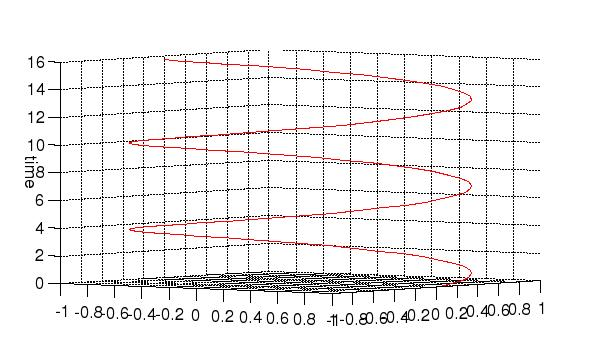
\includegraphics[width=8cm]{zlabel1}}

